\appendix
%\appendixpage
\section*{Appendices}

\section{Performance Rewards with Differentiated Services}

We now describe how the differentiated services
architecture~\cite{blake1998architecture} can be used to improve the control
over traffic priority in Tor, as previously outlined by
Jansen~\cite{jansenphdthesis}. More specifically, the proportional
differentiation model~\cite{dovrolis1999case} allows for predictable (i.e.,
consistent as load increases) and controllable (i.e., adjustable differentiation) performance between N traffic
classes. The model allows for the configuration of a differentiation parameter
$p_i$ for each class $i$, and enforces the proportional priority of a traffic
quality metric $q$ between all pairs of classes $i$ and $j$ for measurement
timescale $\sigma$ as:
\begin{equation}
\forall i \in [N], \forall j \in [N]: \frac{q_i \left( t, t + \sigma \right)}{q_j \left( t, t + \sigma \right)} = \frac{p_i}{p_j}
\end{equation}
where $p_1 < ... < p_N$ and $p_i/p_j$ defines the quality proportion between
classes $i$ and $j$. The model is well defined when there is enough
traffic in each class to allow a work-conserving scheduler to meet the desired
proportions.

Dovrolis \etal design a scheduler under the proportional differentiation model
using a queuing delay metric~\cite{dovrolis2002proportional}, which in our case
corresponds to Tor cell waiting times. For class $i$, the quality metric $q_i$
combines the queuing delay $D_i(t)$ of the longest waiting cell with the
long-term average delay $\delta_i(t)$  of all previously scheduled cells at time $t$:
\begin{equation}
q_i(t) = D_i(t) \cdot f + \delta_i(t) \cdot (1-f)
\end{equation}
where $f$ is an adjustable fraction that tunes the schedulers ability to react
to short term spikes in delay. When a scheduling decision is to be made at time $t$,
the longest waiting cell from the class with the maximum priority
$P(t) = q(t)/p(t)$ is chosen and scheduled.


Todo - DRAFT NOTES:

This section will detail the economic model and present any lingering questions. There will be another diagram featuring multiple clients, a PSP, and multiple hosts. The diagram below will go into the software architecture section, under a section called ``system design'', followed by a sentence describing each component. Then we will go into detail on the ephemeral paths and TorCoin design, which are part of the TorCoin Minter. The TorCoin trader, wallet, and exchange are all necessary, but not novel in terms of design, so we will spend little time on those.

TODO: Add component to Client, ``TorCoin Minter'' (?)

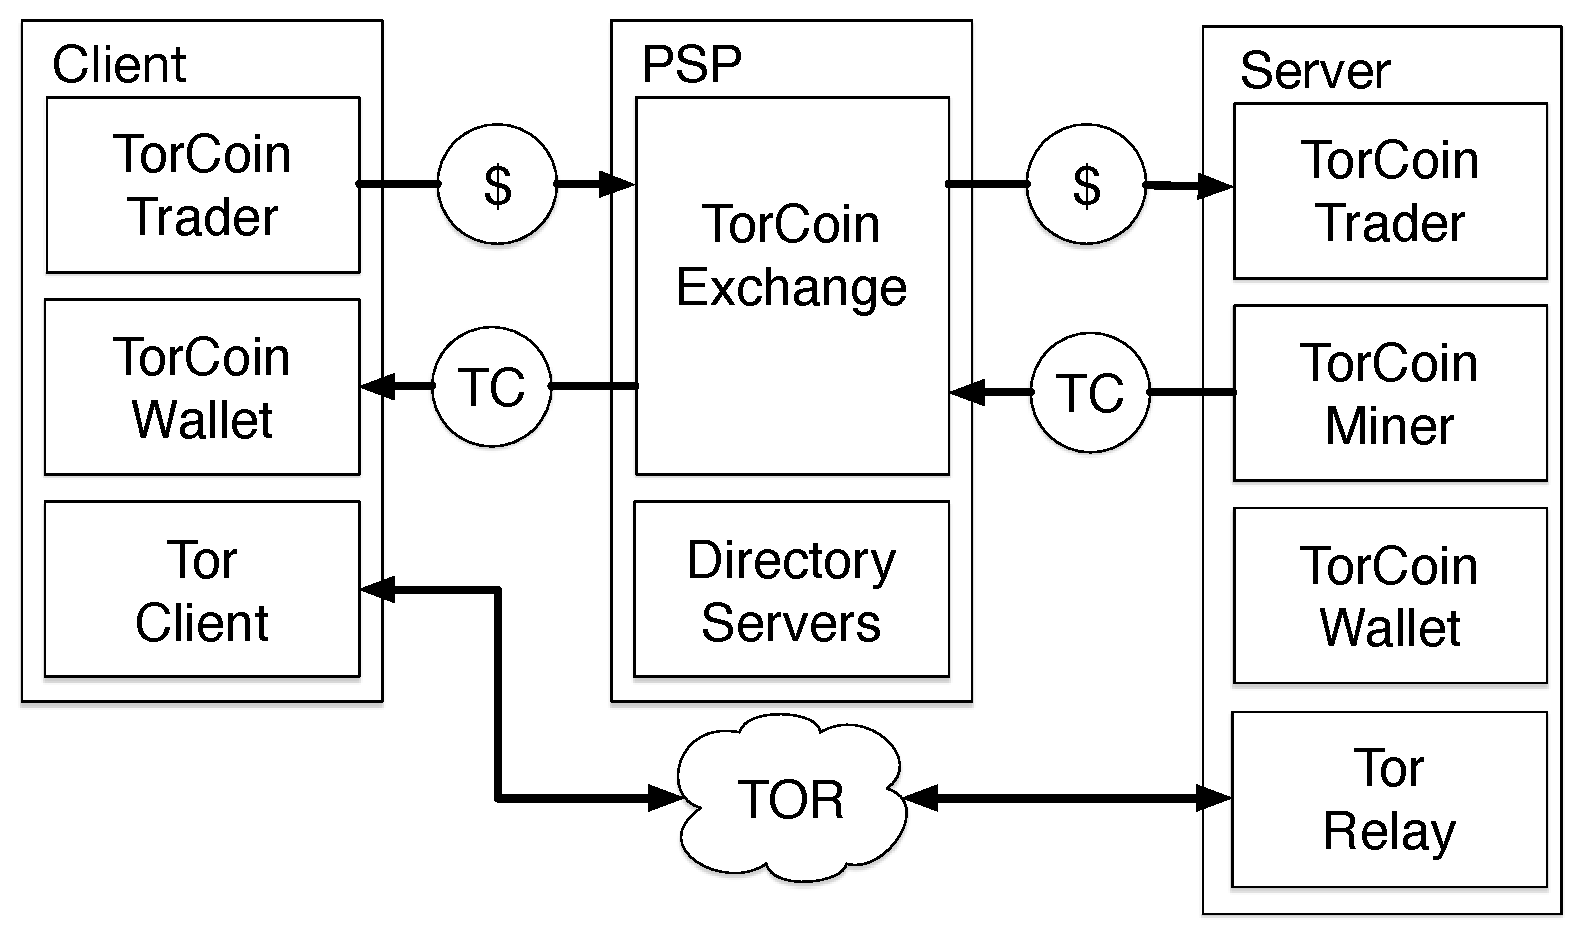
\includegraphics[scale=0.5]{figures/overview.pdf}